\documentclass[12pt]{beamer}

\usepackage{subfigure}
\usepackage{caption}
\usepackage{graphicx}
%\usepackage{natbib}
%\usepackage{bibentry}
\usepackage{biblatex}

\bibliography{refs}

\mode<presentation>
\subtitle{Emden R. Gansner, Yehuda Koren \\ \emph{AT\&T Labs - Research}}
\title{Improved Circular Layouts}
\date{}
\author{Peter Ashwell}

%\newcommand{\newblock}{}

\begin{document}
\maketitle

\begin{frame}
	\frametitle{Overview and Circular Layouts}
	\begin{figure}
	  \centering
	  \subfigure {	
	  	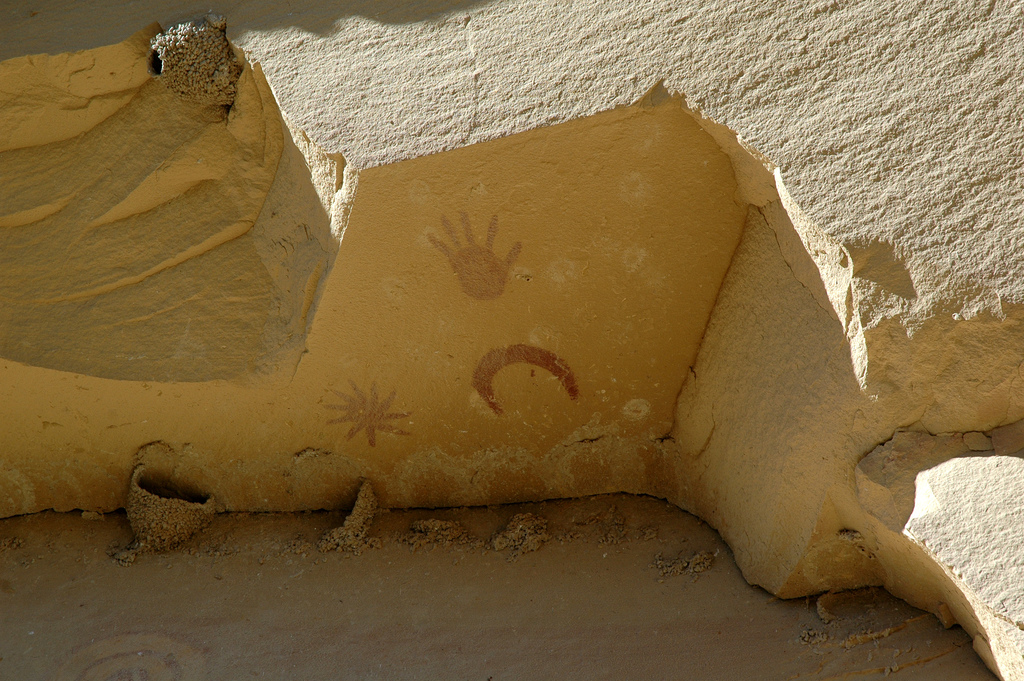
\includegraphics[width=140px]{ccs.jpg}
	  }
	  \subfigure {
	  	\includegraphics[width=140px]{askap.png}
	  }
  	%\caption{Wall painting in Chaco Canyon, NM USA}
	\end{figure}
	Three 

\end{frame}

\begin{frame}
	\frametitle{Time Series Analysis and Gaussian Processes (GPs)}
	\begin{figure}
		\subfigure[Time series of supernova] {
				\captionsetup[subfigure]{labelformat=empty}

			\includegraphics[width=140px]{sne.jpg}
		 }
		\subfigure[GP learning sinc function] {
				\captionsetup[subfigure]{labelformat=empty}

		  	\includegraphics[width=130px]{gp.PNG}
		}
		\captionsetup[subfigure]{labelformat=empty}
	\end{figure}
  Gaussian process: Given some observed mappings from an unknown function $f$: $x \mapsto y$, make predictions about $f$ at unobserved $x_{u}$, or, tell me if some set of other observations were likely to come from $f$.
\end{frame}

\begin{frame}
	\frametitle{Previous Work and the Paper}
	Gaussian processes are computationally and space expensive, both for training and prediction - for $n$ training points:

	\begin{table}
	  \begin{footnotesize}
	  \begin{center}
	  \begin{tabular}{llll}
		Author & Space & Time \\
		Theory, O'Hagan ~\cite{o1978curve} 1978 & - & - \\
		Rasmussen and Williams ~\cite{rasmussen2006gpfml} 2006 & $O(n^{3})$ & $O(n^{2})$ \\
		Various 2001 - 2008  \cite{snelson2005sgppi} \cite{tresp2000bcm} \cite{walder2008sparse} & $O(nm^{2})$ & train $O(nm)$ predict $O(m^{2})$  \\
		This Paper 2010& $O(nm^{2})$ & train $O(nm)$ predict $O(m^{2})$ \\
	  \end{tabular}
	  \end{center}
	  \end{footnotesize}
	\end{table}
	Where $m << n$, $m$ is the number of basis functions in sparse approximation.
	\begin{tiny}
	\begin{enumerate}
		\item \fullcite{o1978curve}
		\item \fullcite{rasmussen2006gpfml}
		\item \fullcite{tresp2000bcm}
		\item \fullcite{snelson2005sgppi}
		\item \fullcite{walder2008sparse}
	\end{enumerate}
	\end{tiny}
\end{frame}

\begin{frame}
  \frametitle{Method}
  \begin{figure}
  	\def \svgwidth{0.85\columnwidth}
  	\input{gproc_fin.pdf_tex}
  \end{figure}
  \begin{tiny}
  \begin{enumerate}
  	\item[6.] A. B. Carlson. Communication Systems. McGraw-Hill, 3rd edition, 1986.
	\item[7.] M. L. Stein. Interpolation of Spatial Data. Springer Verlag, 1999.
  \end{enumerate}
  \end{tiny}
\end{frame}

\begin{frame}
	\frametitle{Paper results and review}
	\begin{itemize}
		\item Evaluation shows slight improvement in accuracy over other sparse methods
		\item Small sacrifice in accuracy over full $O(n^{2})$ GP
		\item More vulnerable than other GP methods to overfitting
	\end{itemize}
	\begin{figure}
	\subfigure{
		\includegraphics[width=150px]{eval3.PNG}
	}
	\end{figure}
\end{frame}

\begin{frame}
  \frametitle{Paper results and review}
		\begin{itemize}
			\item Attractive theoretical computational bounds $O(m^{2})$ for large amounts of data analysis
			\item Respected, well cited experts in GP field and published in highly ranked journal
			\item Evaluation does not discuss exact run-times compared to other sparse methods
			\item Otherwise, rigorous evaluation shows an effective tool for multi-dimensional data modelling
		\end{itemize}
\end{frame}

\begin{frame}
	\frametitle{Research Approach}
	\begin{enumerate}
	  \item Simulate astronomical data 
	  \item Decide on a method to rapidly identify transients, with confidence (perhaps this approach)
	  \item Implement and evaluate method using simulated data
	  \item Expand implementation to large data streams if possible
	\end{enumerate}
%	\cite{tresp2000bcm}
\end{frame}

\begin{frame}
	\frametitle{Thanks!}
	\begin{itemize}
		\item Search for "gaussian process applet" for a fun interactive introduction.
		\item If you're interested in GPs have a read of \emph{Gaussian Processes for Machine Learning} by Rasmussen and Williams (free!)
	\end{itemize}
\end{frame}
%\bibliography{refs}{}
%\bibliographystyle{plain}
\end{document}
